% Advances in Atmospheric Sciences -- manuscript prepared with the AAS LaTeX template
% (AsampleLATEX.zip, https://www.iapjournals.ac.cn/aas/AuthorGuide). Compile with pdfLaTeX.
% Yellow highlights (\todo / \todobox) mark items the authors still have to supply or confirm.
% v8 (2026-09-26): text-only revision around PS-PaE-Fuse as the proposed model; figures unchanged.
\documentclass[12pt]{article}
\usepackage{atmosphere}
\newenvironment{Exercises}[1][10.]{
\refbt{REFERENCES}
\begin{list}
{\hfill }{
\settowidth{\labelwidth}{\bfseries #1}%
\setlength{\labelsep}{0pt}%
\setlength{\topsep}{0bp}%
\setlength{\partopsep}{0pt}%
\setlength{\parskip}{0pt}%
\setlength{\itemsep}{0bp}%
\setlength{\leftmargin}{\labelwidth+\labelsep}%
\usecounter{enumi}}}{\end{list}\smallskip}

\def\tablename{\bf Table}
\def\figurename{\bf Fig.~}

\newcommand{\refbt}[1]{\centering #1}

\def\acknowledgmentsname{{\it Acknowledgements}.\ }

\newcommand{\add}[1]{\vspace*{-19mm}\begin{center}{\small\it #1}\end{center}}

\newcommand{\keywords}[1]{
\begin{center}
\parbox[t]{153mm}{\noindent{\bf Keywords:}\ #1}
\end{center}}

\newcommand{\abs}[1]{\vspace*{-5mm}
\begin{center}
{\bf ABSTRACT}
\end{center}
\vspace*{-5mm}

#1}

\newcommand{\bte}[1]{\vspace*{3mm}\noindent #1}


\setlength{\parskip}{0mm}
\setlength{\arraycolsep}{0.5mm}

\makeatletter
\newskip\@footindent
\@footindent=2.5mm

\renewcommand\footnoterule{\kern6\p@ \hrule width 0.4\columnwidth \kern4\p@}
\@addtoreset{footnote}{page}

\renewcommand\thesection{\arabic{section}.}
\renewcommand\thesubsection{\arabic{section}.\arabic{subsection}}
\renewcommand\thesubsubsection{\arabic{section}.\arabic{subsection}.\arabic{subsubsection}}

\titleformat{\section}{\bf\normalsize}{\thesection}{.5em}{}
\titlespacing{\section}{0mm}{5mm}{0mm}

\titleformat{\subsection}{\bf\normalsize\it}{\thesubsection}{1em}{}
\titlespacing{\subsection}{0mm}{3mm}{0mm}

\titleformat{\subsubsection}{\normalfont\normalsize\it}{\thesubsubsection}{1em}{}
\titlespacing{\subsubsection}{0mm}{3mm}{0mm}

\titleformat{\paragraph}{\normalfont\normalsize\it}{\thesubsubsection}{1em}{}
\titlespacing{\subsubsection}{0mm}{3mm}{0mm}



\linespread{2} 
\usepackage{soul}
\usepackage{xurl}
\newcommand{\fitTable}[1]{\begingroup\linespread{1}\selectfont\setbox0=\hbox{#1}\ifdim\wd0>\linewidth\resizebox{\linewidth}{!}{\box0}\else\box0\fi\endgroup}
\sethlcolor{yellow}
\newcommand{\todo}[1]{\hl{#1}}
\newcommand{\todobox}[1]{\par\noindent\colorbox{yellow}{\parbox{\dimexpr\linewidth-2\fboxsep\relax}{\small #1}}\par}
\newcommand{\mps}{m s$^{-1}$}
\graphicspath{{figures/}}
\renewcommand{\topfraction}{0.9}\renewcommand{\bottomfraction}{0.8}\renewcommand{\textfraction}{0.07}\renewcommand{\floatpagefraction}{0.7}

\begin{document}

\title{\vspace*{-20mm}\fontsize{12}{12}\bf
Extreme-Aware Fusion of Multi-Model AI Weather Forecasts: Joint Optimization of Overall Skill and Event Detection
\vspace*{-3mm}}

\date{}

\author{\\[-17mm]\fontsize{12}{12}
\colorbox{yellow}{First AUTHOR}\footnote{\setlength{\baselineskip}{12pt}Corresponding author: \colorbox{yellow}{Name}\newline\hspace*{6.2mm}Email: \colorbox{yellow}{email@institution.cn}}$^{*1}$,
\colorbox{yellow}{Second AUTHOR}$^{1}$, and \colorbox{yellow}{Third AUTHOR}$^{2}$}

\maketitle

\add{$^1$\colorbox{yellow}{Affiliation 1, City Postal code, China}\\[-3mm]
$^2$\colorbox{yellow}{Affiliation 2, City Postal code, China}}

\abs{Data-driven global weather models now rival physics-based systems in average skill, but combining them smooths the surface-wind extremes on which warnings depend. We introduce PS-PaE-Fuse, an extreme-aware fusion system for Pangu-Weather, GraphCast, FuXi and the ECMWF high-resolution forecast on the global 0.25$^{\circ}$ grid for six variables at 72--168 h. It couples a global-skill expert with a phase-aware selective expert that routes member information in the spatial and Fourier domains, blends them with a frozen forecast-only selector, outputs the mean, a Gaussian scale and event probabilities, and applies a consensus safeguard that restores the locally strongest member where two members agree on strong wind. All components were frozen on 2020 data before evaluation on 22 dates of late 2021 and 32 sealed dates across 2022. On the sealed sample PS-PaE-Fuse raises the critical success index for local q97.5 wind events from 0.286 for Pangu-Weather to 0.344 and the neighbourhood fractions skill score from 0.603 to 0.678, in every season and in tropical-cyclone, cold-surge and non-tropical high-wind conditions, with 14\% lower U10 error. Before the safeguard its U10 CRPS and Brier score are lower than those of EMOS. Ablations show that the safeguard carries the detection gain, reaching the same score on a member mean, whereas the learned experts provide the fused fields and probabilistic outputs; the gain doubles the alert area to the observed event rate and degrades the Brier score. Event-weighted training of a linear stacking shifts raw detection but is absorbed by the safeguard.}

\vspace*{-10mm}

\keywords{AI weather models; deep learning; multi-model fusion; extreme wind; consensus safeguard; forecast verification}

\vspace*{1mm}

\noindent
{\bf Article Highlights:}

\noindent$\bullet$
PS-PaE-Fuse fuses Pangu-Weather, GraphCast, FuXi and HRES with two learned experts, a phase-aware router and a consensus wind safeguard.

\noindent$\bullet$
On 32 sealed 2022 dates, PS-PaE-Fuse lifts q97.5 wind CSI from 0.29 to 0.34 versus Pangu-Weather in every season and weather type.

\noindent$\bullet$
Before the safeguard, its U10 CRPS and q97.5 Brier score are below EMOS; the safeguard trades part of this skill for detection.

\noindent$\bullet$
Ablations show that the safeguard carries the detection gain, while the learned experts provide the fused fields and probabilistic outputs.

\section{Introduction}
\label{sec:intro}

Data-driven global weather models now produce medium-range forecasts whose average errors rival or beat the ECMWF high-resolution deterministic forecast (HRES). Pangu-Weather (Bi et al., 2023), GraphCast (Lam et al., 2023), FuXi (Chen et al., 2023a), FourCastNet (Pathak et al., 2022), FengWu (Chen et al., 2023b), AIFS (Lang et al., 2024), TianXing (Yuan et al., 2025) and the probabilistic GenCast (Price et al., 2025) are prominent examples, WeatherBench~2 provides a common scoreboard (Rasp et al., 2024), and recent reviews discuss their predictability and scientific use (Mu et al., 2025; Dai et al., 2026). Operational-style assessments confirmed the headline skill (Ben Bouall\`egue et al., 2024) but also found that intensity is underestimated in cyclones and windstorms, fields become smoother with lead time, and rare-event skill depends strongly on the metric (Charlton-Perez et al., 2024; Olivetti and Messori, 2024; Pasche et al., 2025); this has motivated deep-learning corrections of AI tropical-cyclone forecasts (Yuan et al., 2026) and hybrid systems that use AI forecasts as large-scale constraints (Niu et al., 2026). Extreme surface wind is particularly demanding, because the double penalty punishes displaced but correctly intense features (Mass et al., 2002) and because rare events are delicate to evaluate with proper scores (Lerch et al., 2017).

Combining models is the classical remedy for random and systematic error, from multi-model superensembles (Krishnamurti et al., 1999; Hagedorn et al., 2005) to averages of AI models that match the best member (Liu et al., 2024), generative superensembles (Nai et al., 2025) and AI ensembles from perturbed initial conditions (Liu et al., 2025; Li et al., 2026). Averaging, however, is a low-pass filter: wind peaks that members place slightly differently are damped, so a fusion that minimizes mean-square error detects fewer strong-wind events than its best member although it is more accurate on average. Post-processing offers tools for both sides of this tension, from EMOS (Gneiting et al., 2005) and neural post-processing (Rasp and Lerch, 2018; Vannitsem et al., 2021; Schulz and Lerch, 2022) to weighted scoring rules and differentiable verification metrics that emphasize the tail (Lagerquist and Ebert-Uphoff, 2022; Allen et al., 2023; Wessel et al., 2025; Biegert et al., 2026); it has recently been applied to AI weather models (Trotta et al., 2025), and operational services now combine physics-based and AI guidance for severe-weather warnings (Zheng et al., 2026). What is missing is a fusion system for AI weather models that is designed for warnings: one that keeps the multi-variable skill of the fused field, raises the detection of extreme wind, provides probabilistic outputs and states what its detection gain costs.

Here we introduce PS-PaE-Fuse, an extreme-aware multi-model fusion system for AI weather forecasts (Fig.~\ref{fig:arch}). Two convolutional experts, one trained for global skill and one that routes member information by comparing amplitudes and phases in the Fourier domain, are blended by a frozen forecast-only selector into the mean, a Gaussian scale and event probabilities for six variables, and a forecast-time consensus safeguard acts on the surface wind. The system is frozen on 2020 data and verified on 22 dates of 2021 and 32 sealed dates of 2022, stratified by season and weather type, against the four members, their mean and ensemble model output statistics (EMOS). Ablations remove the safeguard, transfer it to the member mean, match the alert frequency by a threshold and remove the explicit routing features, and a companion experiment with a 90-parameter linear stacking asks whether event weighting in the training loss can replace or add to the safeguard.

The contributions are threefold: (i) a single system that turns four AI and physics-based members into deterministic, probabilistic and event outputs and raises the detection of local extreme wind above every member in all seasons and above Pangu-Weather in all three weather types; (ii) an accounting of that gain in alert burden, probabilistic cost and idealized cost--loss value, so that users can choose the operating point; and (iii) ablations that attribute the detection gain to the safeguard and the continuous and probabilistic skill to the learned experts, and show that event weighting in the loss is absorbed once the safeguard is applied.

\section{Data and methods}
\label{sec:methods}

\subsection{Forecast members and verification data}
\label{sec:data}

Four deterministic global forecasts are combined: Pangu-Weather (Bi et al., 2023), GraphCast (Lam et al., 2023), FuXi (Chen et al., 2023a) and ECMWF HRES taken at the exact lead time. All fields are on the 0.25$^{\circ}$ latitude--longitude grid (721 $\times$ 1440 points) for six variables: 2-m temperature (T2M, K), the 10-m wind components (U10 and V10, \mps), mean sea-level pressure (MSL, Pa), 500-hPa geopotential (Z500, expressed as geopotential in m$^{2}$ s$^{-2}$) and 850-hPa temperature (T850, K), at lead times of 72, 120 and 168 h from 00 UTC initializations. ERA5 (Hersbach et al., 2020) at the valid time is the verification reference. Pangu-Weather, HRES and ERA5 are read from WeatherBench~2 (Rasp et al., 2024; data sources in the Data availability statement); forecasts are selected by initialization time and exact lead time, and ERA5 at the corresponding valid time. Lead index and latitude order of the historical 2021 HRES cache were corrected to the exact lead and a common north-to-south order. The 2021--2022 GraphCast arrays were generated with the released 37-pressure-level 0.25$^{\circ}$ research checkpoint trained on ERA5 from 1979 to 2017 (checkpoint SHA-256 \texttt{4e8cf600...d3fbacc}); each 00 UTC forecast was initialized from the $-6$ and 0 h ARCO ERA5 analyses and rolled autoregressively at 6-h resolution, retaining the requested daily leads. The corresponding FuXi arrays used the released short- and medium-range ONNX cascade (SHA-256 \texttt{8f23532f...34f0d3c} and \texttt{45fb061b...526fd8c}), initialized from the $-6$ and 0 h WeatherBench~2 ERA5 analyses in the official 70-channel order; the short model supplied steps 1--20 and the medium model steps 21--28. Relative humidity was clipped as an ERA5 fraction to $[0,1]$ and converted to percent before FuXi inference. Complete filenames, hashes and machine-readable run manifests are deposited with the code. Area-integrated verification uses cosine-latitude weighting. Wind speed is derived from U10 and V10 before any threshold is applied.

\subsection{Samples and frozen protocol}
\label{sec:protocol}

Table~\ref{tab:protocol} summarizes the three samples. Development used 2020 only. The 2021 sample consists of 22 initialization dates every four days from 1 October to 24 December 2021, giving 66 global fields per lead-time set; it had been used in earlier development cycles of the neural system and is therefore a reused external sample rather than an untouched test. The 2022 sample consists of 32 initialization dates sampled every 11 days from January to December 2022 (7, 8, 8 and 9 dates in DJF, MAM, JJA and SON); models, thresholds, event definitions and the evaluation code were hashed and sealed before any comparative 2022 score was computed. Because the sample is sparse, all inference is stated per initialization date, and neither year is presented as a full-year or storm-catalogue evaluation.

\begin{table}[t]
\caption{Samples, systems and controls. Seeds are repeated training realizations and never count as independent weather cases.}
\label{tab:protocol}
\vspace*{2mm}
\centering
\small
\fitTable{\begin{tabular}{p{30mm}p{40mm}p{76mm}}
\hline
Experiment & Sample & Systems and controls \\
\hline
Development & 2020; linear stacking: 273 training, 36 selection and 28 diagnostic dates; PS-PaE-Fuse patch evaluation: 71 dates, 1988 tiles & PS-PaE-Fuse global-skill and selective experts; safeguard rule selected among 48 candidates; EMOS; shared Gaussian scale; ridge-initialized linear stacking with $\lambda\in\{0, 0.15, 1.5, 3.18\}$, three seeds each \\
Cross-year test of PS-PaE-Fuse & 22 dates of 2021 (1 Oct--24 Dec, 72/120/168 h); 32 sealed dates of 2022 (every 11 days) & Frozen PS-PaE-Fuse, three router seeds, with and without its consensus safeguard (local q95 trigger, two-member support, $\alpha=1$); Pangu-Weather, GraphCast, FuXi, HRES; simple mean with and without safeguard; development-matched alert-frequency control; locally strongest member; EMOS \\
Objective experiment (linear stacking) & Same 22 dates of 2021 & Twelve frozen linear checkpoints, raw and with a common safeguard (15 \mps\ trigger, $\alpha=0.75$); ridge stacking and simple mean with the same safeguard; four members \\
\hline
\end{tabular}}
\end{table}

\subsection{PS-PaE-Fuse}
\label{sec:model}

PS-PaE-Fuse (Phase-Selective Phase-Aware Ensemble Fusion; Fig.~\ref{fig:arch}) combines two experts in the spirit of a mixture of experts (Jacobs et al., 1991) and adds a consensus safeguard, with 558\,239 deployable parameters. Both experts operate on 96 $\times$ 96 tiles of the four members: a global-skill expert (277\,670 parameters) and a selective expert that routes between candidate combinations using forecast-only features (280\,569 parameters). Both compute member deviations and spread, a 48-channel interaction representation, and a 16-channel context branch using the member fields, orography, land--sea mask and subgrid orography. A 32-channel adaptive router produces a spatial correction, followed by regression refinement and heads for the mean, a positive Gaussian scale and three event logits per variable. Latitude, longitude and lead-time information enter a spherical context module (spherical-harmonic degree 4 and eight latitude radial-basis functions).

The selective expert additionally averages each tile to 48 $\times$ 48, applies a real two-dimensional Fourier transform, and predicts member weights with a 13--16--1 multilayer perceptron. Its inputs are relative log-amplitude, cosine and sine of phase relative to the member consensus, complex disagreement, radial frequency, and four-dimensional lead and member--variable embeddings. Softmax weights mix the complex member coefficients; inverse transformation and bilinear upsampling give a spectral correction. A 72--32--6 convolutional sigmoid gate blends spatial and spectral corrections using interaction features, spread, correction magnitude, coherence and the event-head signal. The deployed router-only variant is trained with a Gaussian-CRPS loss together with focal (Lin et al., 2020) and Tversky (Salehi et al., 2017) event losses, so that overall skill and event detection enter one objective; the optional frequency and high-pass losses shown for the full configuration in Fig.~\ref{fig:arch} are disabled. The archived router launches specify at most 35 epochs, batch size 64, AdamW (Loshchilov and Hutter, 2019) with learning rate $5\times10^{-4}$ and early-stopping patience 10, with three shuffle seeds (123, 456 and 789) sharing one frozen global-skill checkpoint. That checkpoint was retrained from scratch after rebuilding the corrected temporal/U10 cache, using seed 123, base width 32, batch size 64, a maximum of 35 epochs and 7\,840 training plus 1\,988 validation tiles; 6\,760 extreme tiles were repeated three times, producing 21\,360 training samples per epoch. Its latitude-weighted objective combined Gaussian CRPS with focal and Tversky event losses under the archived three-stage event-weight schedule. The lowest validation loss (0.2984) occurred at epoch 16 and that saved state, SHA-256 \texttt{9f1f1ce6...cf07016}, is the frozen global-skill checkpoint used by all router runs; later recorded epochs did not improve it. The complete launch, epoch log and checksum manifest are included in the public repository.

A frozen, parameter-free selector blends the two experts continuously. For each variable, let $a_g$ and $a_p$ be their absolute anomalies from the frozen training climatology, divided by the event scale. The selector is $g=\mathrm{sigmoid}[12(\max(a_g,a_p)-1)]\,\mathrm{sigmoid}[80(a_p-a_g)]$ and returns $\hat y_g+g(\hat y_p-\hat y_g)$, with the same blend applied to Gaussian scale and event logits. In the variable order above, the climatology is $(284.86,0.04,0.19,101051.80,55100.46,279.33)$ and the event scales are $(8,8,7,1200,3000,7)$ in each variable's physical units; verification targets do not enter this selector.

The consensus safeguard acts on the fused wind vector: where at least two members exceed the local 2020 q95 wind-speed threshold, the fused U10 and V10 are replaced by those of the locally strongest member ($\alpha = 1$, no additional speed margin). The rule was selected among 48 candidates on 2020 development tiles and then frozen; it uses forecast information only and leaves the other variables untouched. The complete system, including the safeguard, is referred to as PS-PaE-Fuse; the same system without the safeguard is reported as an ablation, and its outputs are treated as a distinct evaluation object throughout. For probabilistic verification the safeguarded wind is dressed with a Gaussian scale multiplied by a single shared factor of 1.6, chosen on 2020 by blocked cross-validation among 21 values between 0.5 and 2.5 to minimize an equally weighted combination of relative CRPS and Brier score. An EMOS baseline (Gneiting et al., 2005) fitted on 2020 provides the reference probabilistic forecast, and the wind-speed probabilities of the older systems use the delta approximation of independent Gaussian components.

\begin{figure}[tbp]
\centering
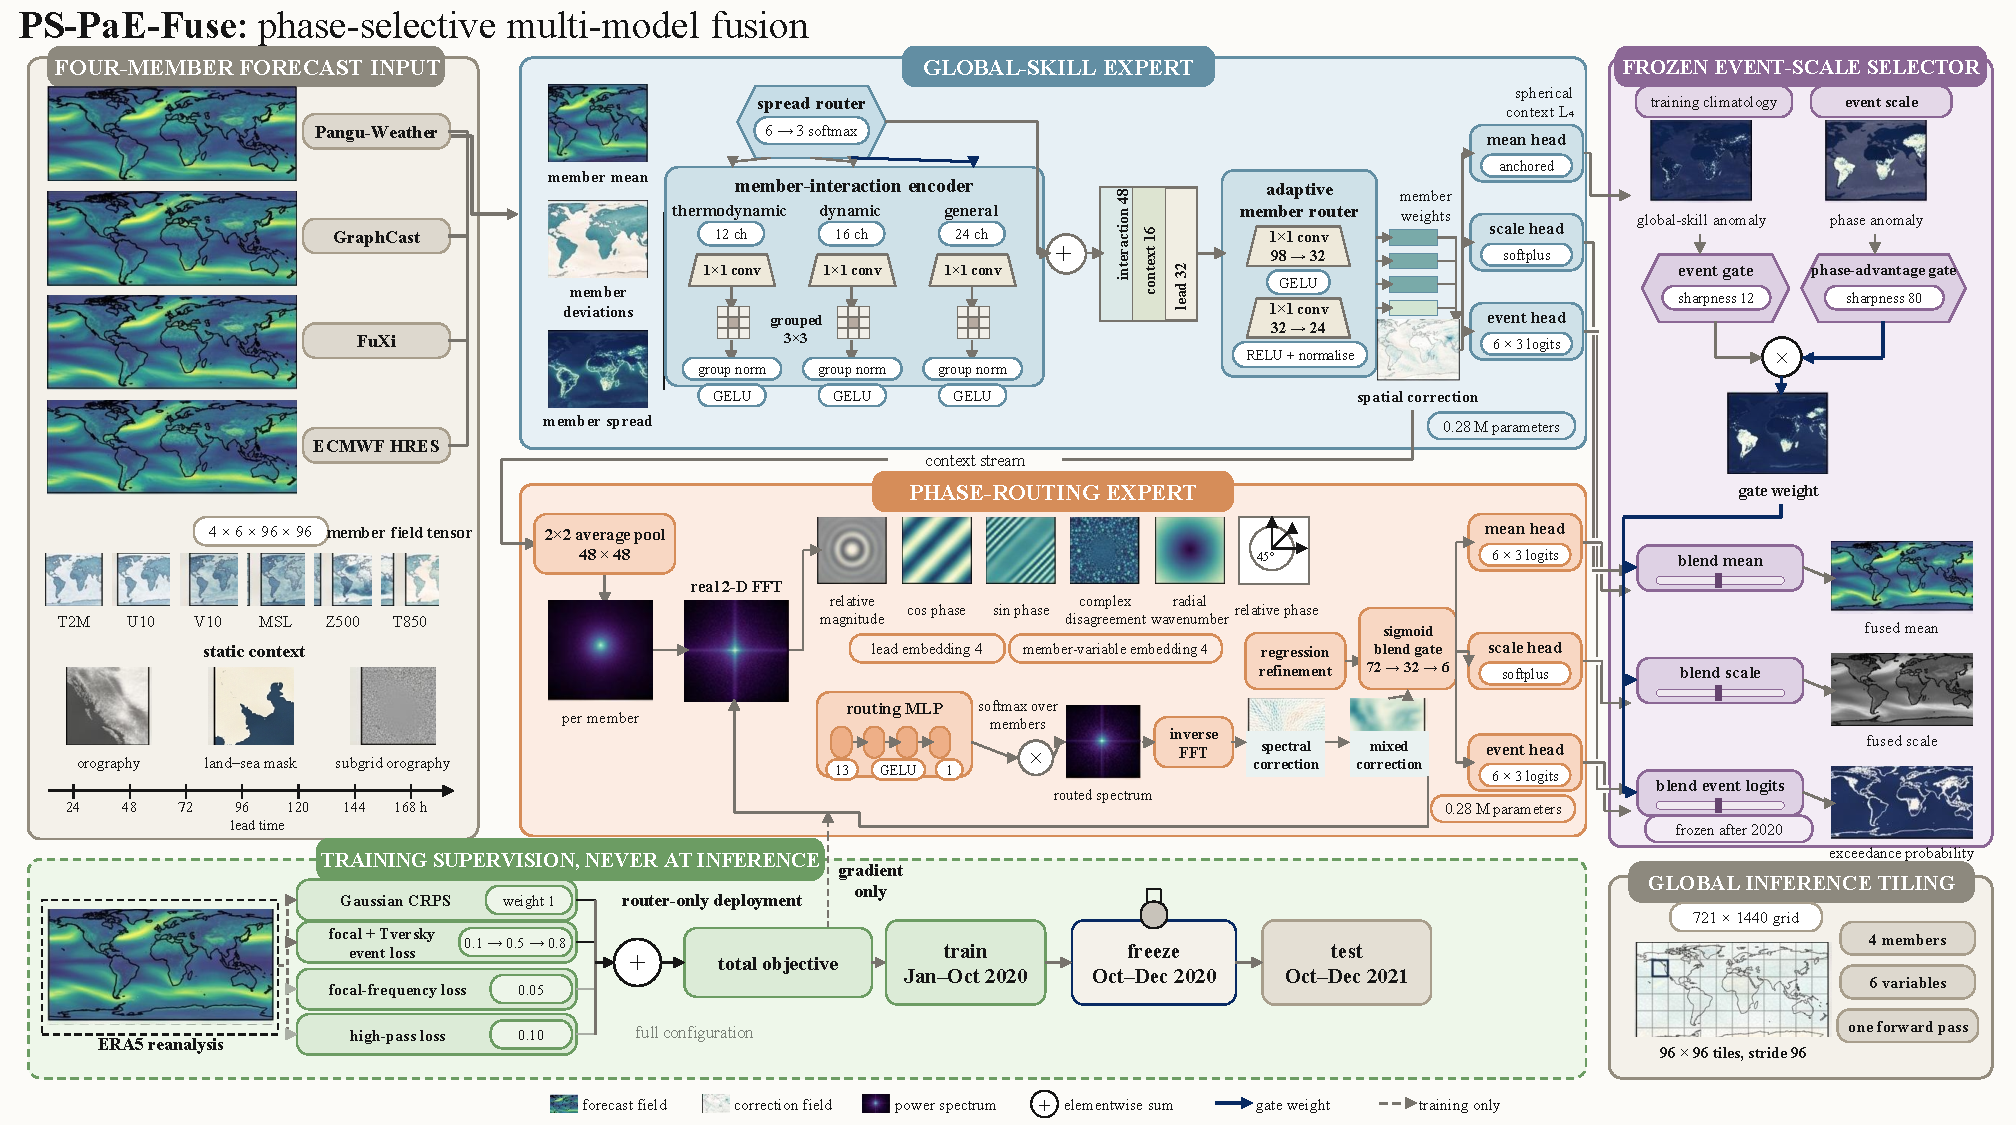
\includegraphics[width=\textwidth]{fig_architecture_ai.pdf}
\caption{Architecture of PS-PaE-Fuse. Four member forecasts enter a global-skill expert and a phase-routing (selective) expert, and a frozen forecast-only event-scale selector blends them into the mean, scale and event outputs. The consensus safeguard (Section~\ref{sec:model}) acts on the fused wind vector downstream of the selector and is not drawn. The 90-parameter linear stacking of the objective experiment (Section~\ref{sec:linear}) uses the same inputs and is not part of PS-PaE-Fuse.}
\label{fig:arch}
\end{figure}

\subsection{Objective experiment with a linear stacking}
\label{sec:linear}

A companion experiment tests whether detection can be obtained through the training objective rather than through a forecast-time rule. A 90-parameter linear stacking corrects the arithmetic member mean with four member coefficients and one bias for each variable and lead time, and is trained with
\begin{equation}
L_{\lambda} = \mathrm{nMSE} + \lambda\,\bigl(1 - \mathrm{CSI}^{\mathrm{soft}}_{20}\bigr),
\label{eq:joint}
\end{equation}
where nMSE is the latitude-weighted mean-square error normalized by the training-only error of the member mean and $\mathrm{CSI}^{\mathrm{soft}}_{20}$ is a differentiable critical success index for 20 \mps\ wind. Four weights ($\lambda = 0$, 0.15, 1.5 and the gradient-calibrated 3.18), with three seeds each, start from the same ridge initialization, are selected on 2020 by the common functional $Q = \mathrm{nMSE} + 0.15\,(1 - \mathrm{CSI}_{20})$, and are frozen and evaluated on 2021 on their raw output and after a common safeguard (15 \mps\ trigger, blending weight $\alpha = 0.75$) that is also applied to the ridge initialization and the simple mean. This rule differs from the PS-PaE-Fuse safeguard, so the two are separate experiments rather than one ablation ladder; the full specification is given in the supplement.

\subsection{Verification}
\label{sec:verif}

Overall skill is measured by nMSE and by per-variable RMSE. Event detection uses contingency scores for wind speed at fixed thresholds of 15, 20 and 25 \mps\ and at local grid-point quantile thresholds (q95 and q97.5) fitted from ERA5 using only fit-day indices 0--219 of 2020, stored separately for 72, 120 and 168 h with the frozen model archive. The critical success index is CSI $= H/(H+M+F)$, probability of detection POD $= H/(H+M)$ and false-alarm ratio FAR $= F/(H+F)$, where $H$, $M$ and $F$ are latitude-weighted hits, misses and false alarms pooled over dates within each lead time (Schaefer, 1990; Wilks, 2011); they are displayed in performance diagrams (Roebber, 2009). Spatial tolerance is assessed with the fractions skill score over a $9\times9$-grid-cell neighbourhood (FSS$_{9}$; Roberts and Lean, 2008), with periodic longitude boundaries. Probabilistic quality uses the proper Gaussian CRPS of U10 and the Brier score of q97.5 exceedance (Brier, 1950; Gneiting and Raftery, 2007). The alert burden is the latitude-weighted fraction of grid cells with a forecast exceedance, compared with the observed event rate, and the idealized economic value follows the cost--loss framework of Richardson (2000) and Murphy (1977): with protection cost $C$, loss $L=1$ and $r=C/L$, the expense per unit opportunity is $E = r\,(H+F)/N + M/N$.

Scores are averaged over the three lead times with equal weight. Uncertainty is estimated by resampling initialization dates with replacement (2\,000 draws for the objective experiment, 5\,000 for PS-PaE-Fuse) with the same draws for all systems, so that intervals of differences are paired; adjacent-date-pair and 7- and 14-day calendar blocks are used as sensitivity checks (Wilks, 1997). Intervals are pointwise sensitivity intervals of a sparse reused sample and are not corrected for multiple comparisons or for the earlier development use of the years. The three seeds are averaged within each date before resampling.

\subsection{Weather-type stratification and cases}
\label{sec:strata}

The 32 sealed 2022 dates are stratified with definitions fixed independently of model performance. Tropical-cyclone (TC) neighbourhoods are the grid cells within 500 km of IBTrACS v04r01 storm centres at the valid time (Knapp et al., 2010), with each storm identifier as the resampling unit (92 storms, of which 81 contain a q97.5 event). Cold-surge cells are those where ERA5 T2M fell by at least 6 K over the preceding 48 h and lies below the pre-2022 local 5th percentile at the valid time; non-tropical high wind is ERA5 wind at or above both the local q97.5 threshold and 20 \mps\ outside all TC masks; for both, the initialization date is the resampling unit (32 dates). Categorical scores in the non-TC stratum are computed over the whole non-TC domain, so its event definition and error support differ from the two other strata. The case maps of Figs.~\ref{fig:weather} and \ref{fig:cases} were selected by the largest truth-only event area within each stratum, never by model performance.

\todo{AAS policy: document here any use of large language models in preparing the manuscript, or confirm that none was used.}

\section{Results}
\label{sec:results}

\subsection{Overall performance of PS-PaE-Fuse}
\label{sec:overall}

Table~\ref{tab:safeguard} summarizes the surface-wind scores of PS-PaE-Fuse and all baselines, and Fig.~\ref{fig:seasonal}e--h shows the 2022 scorecard. In the 2021 sample the configuration without safeguard has the lowest U10 RMSE of all systems (2.043 \mps\ against 2.458 for Pangu-Weather and 2.055 for the simple mean), but its CSI for q97.5 events, 0.288, is below Pangu-Weather (0.301), and its FSS$_{9}$ of 0.569 is below the 0.624 of Pangu-Weather: the fused field is more accurate on average and less sharp on extremes. The complete PS-PaE-Fuse reverses the second half of that statement. It raises the q97.5 CSI to 0.352 (POD from 0.326 to 0.526, FAR from 0.280 to 0.494), the FSS$_{9}$ to 0.683 and the 20 \mps\ CSI to 0.200, while U10 RMSE increases from 2.043 to 2.086 \mps, still 15\% below Pangu-Weather. The gain is threshold-specific: at 15 and 25 \mps\ the CSI (0.351, 0.144) stays below Pangu-Weather (0.358, 0.170), because the safeguard fires on local-quantile consensus rather than absolute speed.

The sealed 2022 sample confirms this picture. Over the 32 dates PS-PaE-Fuse reaches a q97.5 CSI of 0.344 against 0.286 for Pangu-Weather, 0.276 for the simple mean, 0.274 without the safeguard, 0.263 for FuXi, 0.248 for HRES, 0.235 for GraphCast and 0.224 for EMOS; FSS$_{9}$ is 0.678 against 0.603 for Pangu-Weather, and the 20 \mps\ CSI is 0.241 against 0.219. Its U10 RMSE, 2.168 \mps, lies 14\% below Pangu-Weather but 2\% above the configuration without safeguard, the simple mean and EMOS, which are indistinguishable at 2.12 \mps. The three router seeds differ in q97.5 CSI by a sample standard deviation of 0.0011 before the safeguard and 0.00003 after it, a consequence of the safeguard frequently replacing the learned wind by the same member; this near-invariance is a property of the safeguard and must not be read as robustness of the learned routing.

\begin{table}[t]
\caption{Surface-wind scorecard of PS-PaE-Fuse and all baselines on the 2021 sample (22 dates) and the sealed 2022 sample (32 dates), equal-lead means; PS-PaE-Fuse rows are three-seed means. U10 RMSE is the RMSE of the zonal component; CSI, POD, FAR and FSS$_{9}$ refer to wind-speed events at the local q97.5 threshold; CSI$_{20}$ to 20 \mps. Member FSS$_{9}$ in 2021 is from the archived raw-member evaluation; dashes mark scores not archived for that system.}
\label{tab:safeguard}
\vspace*{2mm}
\centering
\small
\fitTable{\begin{tabular}{llcccccc}
\hline
Sample & System & U10 RMSE & CSI & POD & FAR & FSS$_9$ & CSI$_{20}$ \\
 & & (m s$^{-1}$) & q97.5 & q97.5 & q97.5 & q97.5 & 20 m s$^{-1}$ \\
\hline
2021 (22 dates) & Pangu-Weather & 2.458 & 0.301 & 0.398 & 0.468 & 0.624 & 0.182 \\
 & GraphCast & 2.262 & 0.268 & -- & -- & 0.557 & 0.163 \\
 & FuXi & 2.191 & 0.270 & -- & -- & 0.545 & 0.162 \\
 & ECMWF HRES & 2.745 & 0.251 & -- & -- & 0.597 & 0.155 \\
 & Simple mean & 2.055 & 0.290 & -- & -- & 0.577 & 0.167 \\
 & PS-PaE-Fuse w/o safeguard & 2.043 & 0.288 & 0.326 & 0.280 & 0.569 & 0.163 \\
 & PS-PaE-Fuse & 2.086 & 0.352 & 0.526 & 0.494 & 0.683 & 0.200 \\[5pt]
2022 (32 dates) & Pangu-Weather & 2.530 & 0.286 & 0.378 & 0.477 & 0.603 & 0.219 \\
 & GraphCast & 2.386 & 0.235 & 0.270 & 0.379 & 0.509 & 0.145 \\
 & FuXi & 2.290 & 0.263 & 0.317 & 0.362 & 0.541 & 0.162 \\
 & ECMWF HRES & 2.797 & 0.248 & 0.477 & 0.664 & 0.598 & 0.186 \\
 & Simple mean & 2.128 & 0.276 & 0.313 & 0.289 & 0.564 & 0.172 \\
 & EMOS & 2.124 & 0.224 & 0.244 & 0.228 & 0.466 & 0.128 \\
 & PS-PaE-Fuse w/o safeguard & 2.123 & 0.274 & 0.310 & 0.281 & 0.557 & 0.161 \\
 & PS-PaE-Fuse & 2.168 & 0.344 & 0.517 & 0.495 & 0.678 & 0.241 \\
\hline
\end{tabular}
}
\end{table}

\begin{figure}[tbp]
\centering
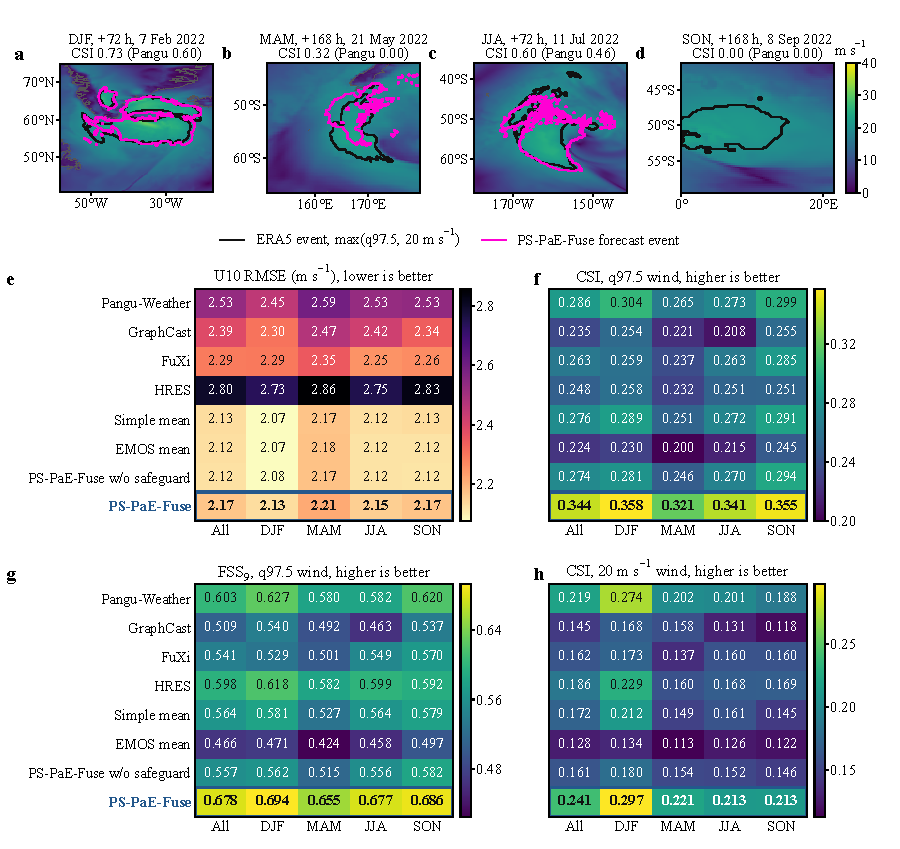
\includegraphics[width=\textwidth]{fig_seasonal_2022.pdf}
\caption{Seasonal context and all-system scorecard on the sealed 2022 sample (32 initialization dates: 7/8/8/9 in DJF/MAM/JJA/SON). (a--d) Truth-selected seasonal cases distinct from Figs.~\ref{fig:weather} and \ref{fig:cases}: ERA5 wind with the observed (black) and PS-PaE-Fuse (magenta) max(q97.5, 20 \mps) events; titles give the sector CSI of PS-PaE-Fuse and Pangu-Weather. (e--h) Equal-lead means over 72, 120 and 168 h for U10 RMSE, local-q97.5 CSI and FSS$_9$, and 20 \mps\ CSI. The outlined row is PS-PaE-Fuse; PS-PaE-Fuse rows are three-seed means.}
\label{fig:seasonal}
\end{figure}

\subsection{Consistency across seasons and weather types}
\label{sec:consistency}

The detection gain holds in every season (Fig.~\ref{fig:seasonal}f): the q97.5 CSI of PS-PaE-Fuse is 0.32--0.36, against 0.27--0.30 for Pangu-Weather in the same seasons (Table~S5). Fig.~\ref{fig:weather} stratifies the same 32 dates by weather type; the full paired table is Table~S4 and results by lead are in Fig.~S2. Relative to Pangu-Weather, PS-PaE-Fuse improves the q97.5 CSI in all three strata: $+0.042$ [$+0.017$, $+0.067$] within 500 km of the 92 tropical cyclones, $+0.053$ [$+0.023$, $+0.093$] in cold-surge cells and $+0.036$ [$+0.019$, $+0.053$] for non-tropical high wind, with FSS$_{9}$ and POD gains in every stratum (Table~S4). PS-PaE-Fuse has the higher CSI for 49 of 81 storms with events and for 24 and 26 of the 32 cold-surge and non-TC dates (Fig.~\ref{fig:weather}g--i). The false-alarm ratio is unchanged in the TC and cold-surge strata (intervals cross zero) but rises by $+0.089$ [$+0.059$, $+0.120$] for non-tropical high wind, whose events use the stricter max(q97.5, 20 \mps) criterion over the whole non-TC domain. U10 RMSE conditional on event cells improves in the cold-surge ($-0.55$ \mps) and non-TC ($-0.36$ \mps) strata but not for tropical cyclones ($+0.16$ \mps, interval crossing zero), where the safeguard restores the Pangu-Weather core and inherits its position errors.

Relative to the configuration without safeguard the CSI gains are larger ($+0.172$, $+0.035$ and $+0.076$, the cold-surge interval crossing zero), and so are the costs: FAR rises by $+0.136$, $+0.199$ and $+0.410$, U10 RMSE and CRPS on event cells worsen in the TC ($+0.55$ and $+0.14$ \mps) and cold-surge ($+0.08$ and $+0.03$ \mps) strata (RMSE in Fig.~\ref{fig:weather}g, h), and the q97.5 Brier score worsens in the cold-surge and non-TC strata while improving for tropical cyclones (Table~S4). For Malakas the core peaks at 26.6 \mps\ in ERA5, 26.2 \mps\ in PS-PaE-Fuse and 21.6 \mps\ without the safeguard (Fig.~\ref{fig:weather}a). The context cases of Fig.~\ref{fig:weather}a--c differ from those of Fig.~\ref{fig:cases} and were selected from ERA5 alone before their forecasts were extracted.

\begin{figure}[tbp]
\centering
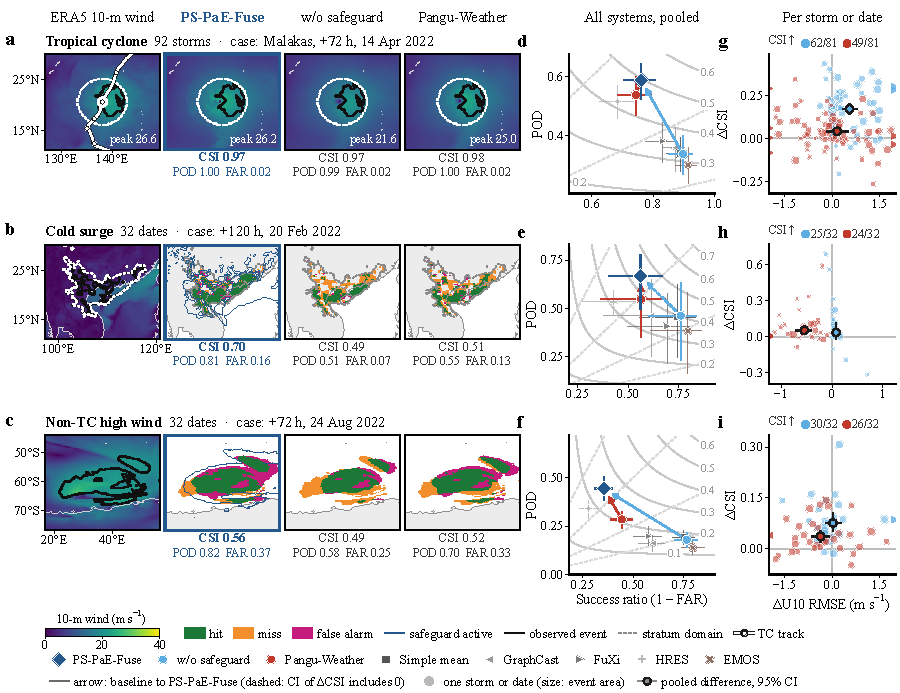
\includegraphics[width=\textwidth]{fig_weather_type_2022.pdf}
\caption{Weather-type cases and stratified verification on the sealed 2022 sample, one row per stratum. (a--c) ERA5-selected cases not used in Fig.~\ref{fig:cases}: ERA5 10-m wind and forecasts of PS-PaE-Fuse, PS-PaE-Fuse without the safeguard and Pangu-Weather, scored in the mapped sector of the stratum domain (dashed). Malakas is shown as wind speed (black: observed $\geq$20 \mps; white: IBTrACS track) because its neighbourhood exceeds the local q97.5 threshold almost everywhere; the other rows show hits, misses and false alarms, with the safeguard-active area outlined. (d--f) Performance diagrams of all systems pooled over 92 storms or 32 dates (95\% intervals; curves: CSI; dashed: frequency bias 0.25--2; arrows dashed where the $\Delta$CSI interval includes zero). (g--i) Per-unit differences of PS-PaE-Fuse from Pangu-Weather (red) and from the configuration without safeguard (blue), with pooled values and 95\% intervals (2\,000 resamples); numbers count units with higher CSI.}
\label{fig:weather}
\end{figure}

\subsection{Case studies}
\label{sec:cases}

Fig.~\ref{fig:cases} compares PS-PaE-Fuse with every deterministic baseline in three truth-selected 2022 cases. PS-PaE-Fuse has the highest grid-cell CSI for Typhoon Nanmadol (0.99; Pangu-Weather 0.97, GraphCast 0.95 and FuXi 0.90) and for the North Atlantic windstorm (0.45; the strongest baseline, GraphCast, 0.43). In the South American cold-surge case it is effectively tied with GraphCast (0.766 versus 0.770) and exceeds Pangu-Weather (0.744). Without the safeguard the same system scores 0.66, 0.76 and 0.33 in the three cases. The fields were selected by observed event geometry alone and illustrate spatial behaviour rather than average performance.

\begin{figure}[tbp]
\centering
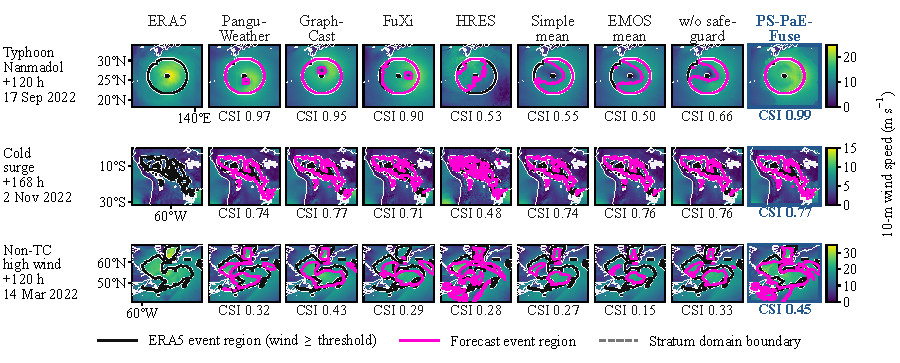
\includegraphics[width=\textwidth]{fig_cases_2022.pdf}
\caption{All-system wind-field comparison for three truth-selected 2022 cases. Rows show Typhoon Nanmadol (+120 h; valid 17 September), a South American cold surge (+168 h; 2 November) and a North Atlantic windstorm (+120 h; 14 March). Columns show ERA5, Pangu-Weather, GraphCast, FuXi, HRES, simple mean, EMOS mean and PS-PaE-Fuse without and with the safeguard (seed 123). Black--white contours mark the observed event, magenta the forecast event and grey dashes the stratum domain; labels report grid-cell CSI.}
\label{fig:cases}
\end{figure}

\subsection{Ablation: contributions of the learned experts and the safeguard}
\label{sec:ablation}

Table~\ref{tab:alert} and Fig.~\ref{fig:decision} decompose the detection gain of PS-PaE-Fuse into its components and compare it with matched controls. On the windstorm date of Fig.~\ref{fig:cases} (Fig.~\ref{fig:decision}a--e) the safeguard covers much of the storm, and PS-PaE-Fuse detects more of the observed area than the simple mean with fewer false alarms than the locally strongest member. Removing the safeguard lowers the alerted area from 3.13\% to 1.31\% of the weighted area, against an observed q97.5 event rate of 3.12\%, and the CSI from 0.344 to 0.274; with the safeguard, POD rises from 0.31 to 0.52 and FAR from 0.28 to 0.50. Replacing the learned experts by the plain member mean, with the same safeguard, reaches the same CSI of 0.344 at the same alert fraction: the paired difference between PS-PaE-Fuse and the safeguarded member mean is $+0.00001$ [$-0.00012$, $+0.00014$] in CSI, with a marginally negative FSS$_{9}$ difference. A post-test exploratory ablation that removes the explicit routing features from the selective expert (three matched seeds) changes the CSI by $+0.0000026$ [$-0.0000036$, $+0.0000095$]. Within PS-PaE-Fuse the detection gain is therefore carried by the safeguard; the learned experts contribute the continuous fields, whose U10 RMSE is 16\% below Pangu-Weather in 2022 and comparable to the member mean, and the probabilistic outputs of Section~\ref{sec:prob}.

Two controls test whether the safeguard is more than a lower alert threshold. A simple mean whose exceedance threshold was scaled on 2020 development fields to match the alert frequency of the safeguarded mean (factors 0.93, 0.91 and 0.90 at 72, 120 and 168 h; Table~S8) reaches a 2022 CSI of 0.342 [0.324, 0.358] at an alert fraction of 3.30\%; the safeguarded mean minus this control is $+0.002$ [$-0.003$, $+0.008$] in CSI and $-0.013$ in FAR. Much of the gain is thus reproducible by a frequency adjustment, but the safeguard reaches it with fewer false alarms, because the substituted member carries spatial information that a uniform threshold does not. The locally strongest member alone has a POD of 0.63 but a FAR of 0.66 and an alert fraction of 5.9\%, so the two-member consensus is what keeps the burden near the event rate (Fig.~\ref{fig:decision}f--h).

The idealized cost--loss valuation of Fig.~\ref{fig:decision}i, j turns these contingency counts into value and expense: near the event rate the relative value is 0.50 for PS-PaE-Fuse, 0.36 for Pangu-Weather and 0.30 for the simple mean. Relative to the simple mean and to Pangu-Weather, the safeguarded simple mean has lower expense for cost--loss ratios below about 0.35 and 0.48 and higher expense above; relative to the frequency-matched control it has lower expense above a ratio of about 0.23, where its lower false-alarm ratio pays, with a pointwise band that crosses zero over a wide range of ratios. The curves use the event rate of the sample as climatological reference and are not estimates of realized economic benefit.

\begin{table}[t]
\caption{Ablation of PS-PaE-Fuse and matched controls on the sealed 2022 sample for local q97.5 wind events, equal-lead means with 95\% paired-date intervals (5\,000 draws); the observed event fraction is 3.12\% of the weighted area. The development-matched control scales the simple-mean exceedance threshold so that its alert frequency on 2020 development fields matches that of the safeguarded mean; it is a decision-threshold control and leaves the continuous field unchanged.}
\label{tab:alert}
\vspace*{2mm}
\centering
\small
\fitTable{\begin{tabular}{llcccc}
\hline
System & Role & CSI [95\% CI] & POD & FAR & Alert area (\%) \\
\hline
PS-PaE-Fuse & Complete system & 0.344 [0.329, 0.359] & 0.517 & 0.495 & 3.13 \\
PS-PaE-Fuse w/o safeguard & Ablation & 0.274 [0.256, 0.291] & 0.310 & 0.281 & 1.31 \\
Member mean + safeguard (experts replaced) & Ablation & 0.344 [0.329, 0.359] & 0.517 & 0.495 & 3.13 \\[5pt]
Simple mean, development-matched alert frequency & Control & 0.342 [0.324, 0.358] & 0.529 & 0.509 & 3.30 \\
Locally strongest member & Control & 0.283 [0.271, 0.295] & 0.632 & 0.665 & 5.91 \\
Simple mean & Control & 0.276 [0.258, 0.293] & 0.313 & 0.289 & 1.34 \\
Pangu-Weather & Member & 0.286 [0.270, 0.300] & 0.378 & 0.477 & 2.24 \\
ECMWF HRES & Member & 0.248 [0.236, 0.260] & 0.477 & 0.664 & 4.40 \\
\hline
\end{tabular}
}
\end{table}

\begin{figure}[tbp]
\centering
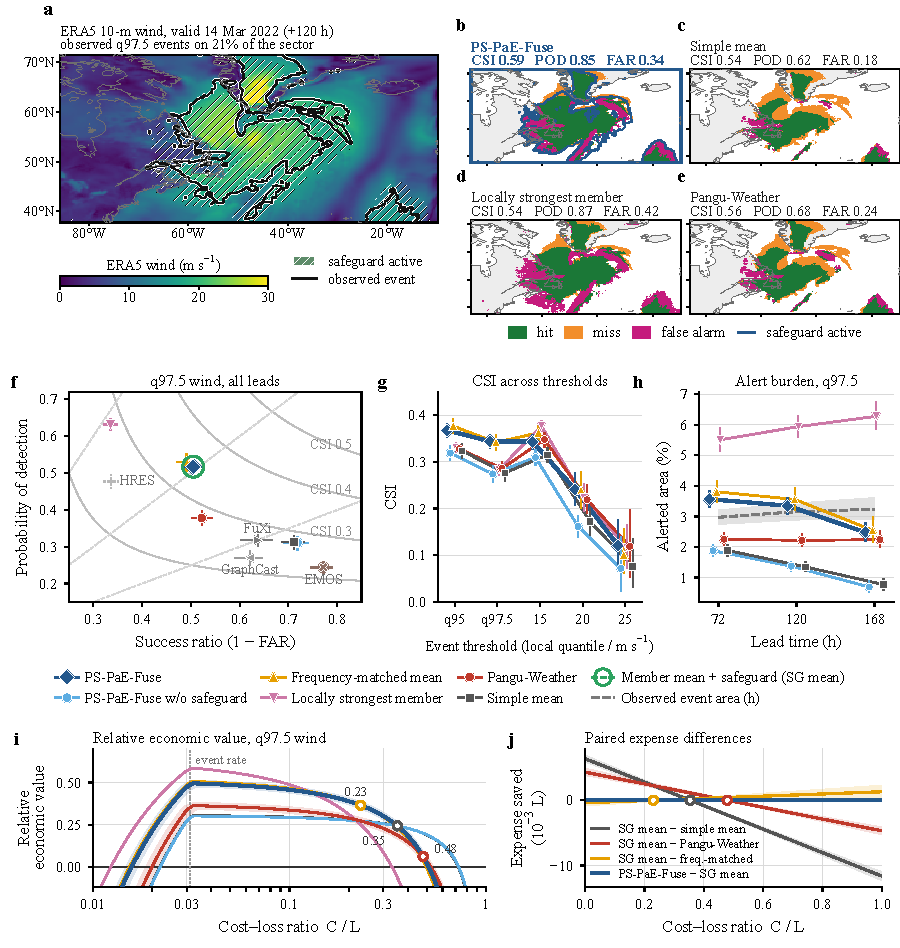
\includegraphics[width=\textwidth]{fig_decision_2022.pdf}
\caption{Detection, alert burden and decision value on the sealed 2022 sample. (a) ERA5 10-m wind, local-q97.5 event region and safeguard-active cells (hatched) on the windstorm date of Fig.~\ref{fig:cases} (+120 h); (b--e) hits, misses and false alarms of four systems on that date and sector. (f) Performance diagram (grey curves: CSI; dashed: frequency bias 0.5, 1, 2), (g) CSI by threshold and (h) alerted area by lead for local-q97.5 events, with 95\% paired-date intervals. (i) Relative economic value (0: sample climatology; 1: perfect) and (j) paired expense differences (SG mean: member mean with safeguard), with 95\% paired-date bands; circles mark break-even ratios.}
\label{fig:decision}
\end{figure}

\subsection{Probabilistic outputs and the six-variable balance}
\label{sec:prob}

The safeguard also changes the probabilistic outputs of PS-PaE-Fuse (Table~\ref{tab:prob}). Before the safeguard PS-PaE-Fuse is the best probabilistic system: its U10 CRPS of 1.003 and q97.5 Brier score of 0.02050 are below the EMOS values of 1.016 and 0.02141. The independent 2021 reliability diagrams show the same lead-dependent comparison (Fig.~\ref{fig:multivarprob}d--f): the three-seed pre-safeguard output has lower Brier score than EMOS at 72, 120 and 168 h, and lower CRPS at 120 and 168 h while the 72-h values are effectively tied. Substituting the strongest member inflates the distribution's centre without adjusting its spread, and the uncalibrated complete system has a CRPS of 1.018 and a Brier score of 0.02352. The single shared scale factor of 1.6 fitted on 2020 recovers part of the loss, to 1.017 and 0.02263, i.e. about one third of the Brier degradation, but the complete system remains worse than the configuration without safeguard and, in CRPS, marginally worse than EMOS. Detection gain and probabilistic loss are two views of the same operating point: users who need the best probabilistic scores can take the outputs before the safeguard, and a conditional calibration of the safeguarded output is a candidate extension, for which a development-set pilot is reported in the supplement only (Table~S9) because it has not been confirmed on external data.

The six-variable balance of the learned experts is modest relative to the already strong member mean (Table~S2), but consistently favourable relative to Pangu-Weather across the three reported leads (Fig.~\ref{fig:multivarprob}a--c). In the corrected 2021 all-grid evaluation, PS-PaE-Fuse without the safeguard improves RMSE over Pangu-Weather for all six variables at 72, 120 and 168 h, by 10.8--20.7\% depending on variable and lead; most of this gain is shared with the simple mean and the global-skill expert. Relative to the simple mean, the equal-lead RMSE of the global-skill expert is lower by 0.008 K for T2M and 0.012 \mps\ for U10 but higher by 0.008 \mps\ for V10, 3.4 Pa for MSL, 3.2 m$^{2}$ s$^{-2}$ for Z500 and 0.009 K for T850, and the three router seeds behave alike. A post hoc stratification by member disagreement finds a T2M skill of $+1.7\%$ [$+0.7\%$, $+2.8\%$] relative to the simple mean in the highest-disagreement tercile but no advantage for the other variables, so PS-PaE-Fuse is not claimed to improve all six variables beyond the simple mean or to have a general advantage under disagreement.

\begin{figure}[tbp]
\centering
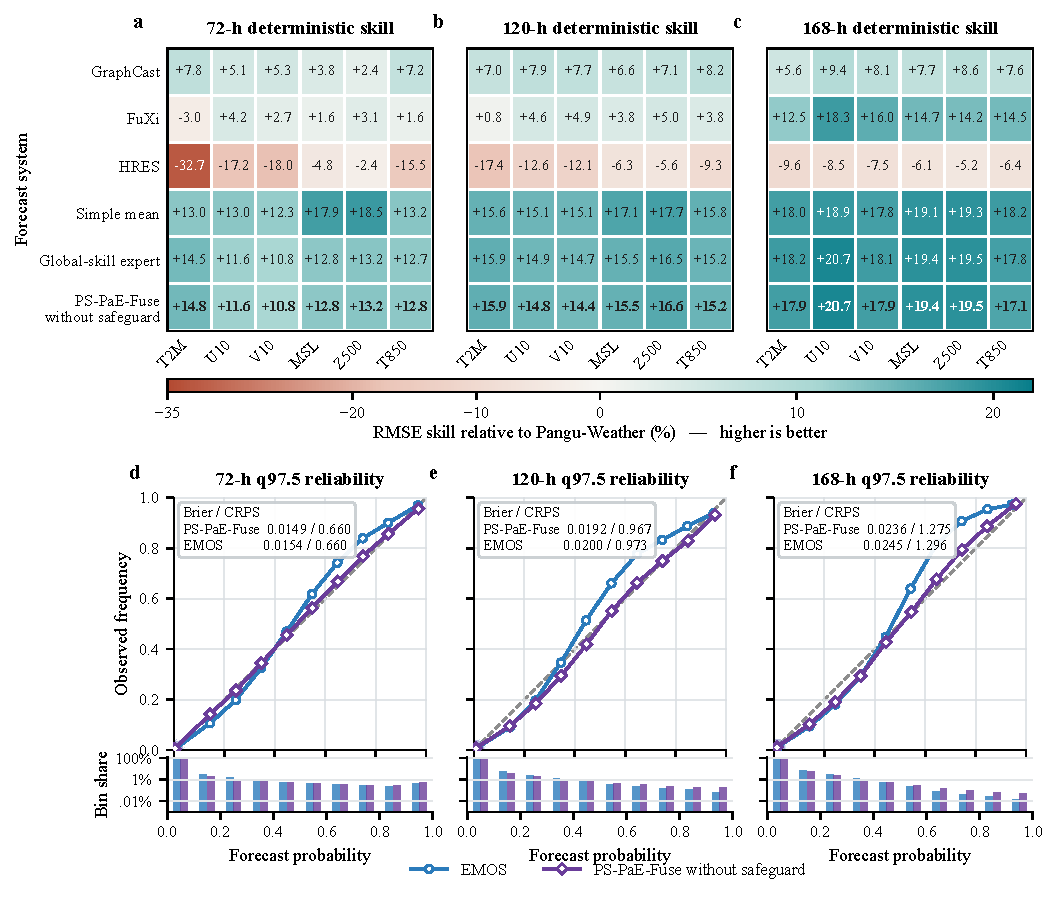
\includegraphics[width=0.84\textwidth]{fig_multivariate_probability_2021.pdf}
\caption{Multi-variable deterministic skill and probabilistic wind verification on the corrected 2021 external sample (22 initialization dates). (a--c) Latitude-weighted all-grid RMSE skill relative to Pangu-Weather, $100(\mathrm{RMSE}_{\mathrm{Pangu}}-\mathrm{RMSE}_{\mathrm{system}})/\mathrm{RMSE}_{\mathrm{Pangu}}$, at 72, 120 and 168 h. The PS-PaE-Fuse row is the three-seed mean before the safeguard. (d--f) Reliability for local-q97.5 wind exceedance from the same output and EMOS; symbol area and lower histograms show bin population, and insets give Brier score and Gaussian U10 CRPS. Thresholds and EMOS parameters were fixed on 2020; wind probabilities use the delta approximation of independent Gaussian components.}
\label{fig:multivarprob}
\end{figure}

\begin{table}[t]
\caption{Probabilistic and deterministic scores of PS-PaE-Fuse and EMOS on the sealed 2022 sample (32 dates, equal-lead means). CRPS is for the Gaussian U10 forecast; the Brier score for local q97.5 wind exceedance. The shared scale factor of 1.6 was fitted on 2020 only. Rows with a single seed are given so that uncalibrated and calibrated values are compared like for like.}
\label{tab:prob}
\vspace*{2mm}
\centering
\small
\fitTable{\begin{tabular}{lcccc}
\hline
System & U10 CRPS & Brier, q97.5 & U10 RMSE & CSI, q97.5 \\
\hline
EMOS & 1.0157 & 0.02141 & 2.124 & 0.224 \\
PS-PaE-Fuse w/o safeguard (three-seed mean) & 1.0027 & 0.02050 & 2.123 & 0.274 \\
PS-PaE-Fuse, uncalibrated scale (seed 123) & 1.0181 & 0.02352 & 2.168 & 0.344 \\
PS-PaE-Fuse, shared scale 1.6 (seed 123) & 1.0168 & 0.02263 & 2.168 & 0.344 \\
PS-PaE-Fuse, shared scale 1.6 (three-seed mean) & 1.0167 & 0.02263 & 2.168 & 0.344 \\
\hline
\end{tabular}
}
\end{table}

\subsection{Event-weighted training and the safeguard}
\label{sec:objective}

The objective experiment of Section~\ref{sec:linear} asks whether detection could instead be obtained by weighting events in the training loss (Table~\ref{tab:joint}; paired differences and interactions in Tables~S10 and S11). On raw output the three joint weights raise the equal-lead CSI$_{20}$ from 0.1465 to 0.1550, 0.1625 and 0.1638 for $\lambda = 0.15$, 1.5 and 3.18, with paired-date intervals from $+0.0085$ [$+0.0056$, $+0.0111$] to $+0.0173$ [$+0.0106$, $+0.0237$], while nMSE changes by less than 0.04\% of the $\lambda=0$ value. The direction holds for every seed, leave-one-date-out subsample and calendar block (Table~S7), and the 2020 diagnostic set shows the same ordering at larger amplitude (Table~S1). The gain is concentrated at 72 and 120 h (Fig.~\ref{fig:objective}h; Fig.~S1), where the joint models forecast stronger winds and both POD and FAR increase; the largest raw RMSE increase is 0.34\% for U10 at 72 h (Table~S3). The raw joint models thus sit between ridge stacking and the simple mean (Table~\ref{tab:joint}; Fig.~S3).

The safeguard absorbs this increment (Fig.~\ref{fig:objective}h, i): the raw joint objectives raise CSI$_{20}$ on 19 of the 22 dates, the safeguarded ones on 11 or 12. The ERA5-selected case of 11 December 2021 (+72 h; Fig.~\ref{fig:objective}a--g) shows how. Event weighting ($\lambda = 3.18$) raises the raw 10-m wind over the observed storm by 0.41 \mps\ and adds hits equal to 4.6\% and false alarms equal to 10.8\% of the event area. The safeguard, active over 98\% of the event cells, moves both objectives towards the same member, so these differences fall to 0.11 \mps, 1.4\% and 4.3\%. After the common rule the joint models reach CSI$_{20}$ of 0.2094, 0.2083 and 0.2082 against 0.2099 for the $\lambda=0$ control, differences of $-0.0005$ to $-0.0016$ whose intervals touch or cross zero, and the interaction (safeguarded minus raw difference) is negative for every weight ($-0.0089$ to $-0.0189$). At 72 h the joint model brings more strong-wind cells into the consensus, and after the substitution more of them are false: for $\lambda = 3.18$ the safeguarded difference splits into $+0.008$ from additional hits and $-0.015$ from additional false alarms (Fig.~\ref{fig:objective}j). The safeguarded ridge stacking dominates all safeguarded joint models in point estimates (not significantly for $\lambda = 0.15$; Table~S10). Event weighting in the loss therefore moves a raw fusion along the skill--detection frontier but adds nothing once a consensus safeguard is applied, consistent with the design of PS-PaE-Fuse, which places detection in a forecast-time module.

\begin{table}[t]
\caption{Frozen 2021 cross-year scores of the objective experiment (22 initialization dates, 72/120/168 h, six variables): the four training objectives of the linear stacking on raw and safeguarded output, three-seed means with the sample standard deviation over seeds in parentheses, together with the matched controls and the four members. nMSE is the training-scale normalized mean-square error, CSI$_{20}$ the equal-lead CSI for 20 \mps\ wind and $Q = \mathrm{nMSE} + 0.15\,(1-\mathrm{CSI}_{20})$ the common selection functional.}
\label{tab:joint}
\vspace*{2mm}
\centering
\small
\fitTable{\begin{tabular}{llccc}
\hline
System & Output & nMSE & CSI$_{20}$ & $Q$ \\
\hline
Overall error only, $\lambda=0$ & Raw & 0.97795 (0.00008) & 0.1465 (0.0004) & 1.1060 \\
Overall error only, $\lambda=0$ & Safeguarded & 0.98363 (0.00008) & 0.2099 (0.0001) & 1.1022 \\
Joint, $\lambda=0.15$ & Raw & 0.97790 (0.00005) & 0.1550 (0.0004) & 1.1047 \\
Joint, $\lambda=0.15$ & Safeguarded & 0.98361 (0.00005) & 0.2094 (0.0000) & 1.1022 \\
Joint, $\lambda=1.5$ & Raw & 0.97823 (0.00010) & 0.1625 (0.0012) & 1.1039 \\
Joint, $\lambda=1.5$ & Safeguarded & 0.98396 (0.00010) & 0.2083 (0.0005) & 1.1027 \\
Joint, gradient-calibrated $\lambda=3.18$ & Raw & 0.97833 (0.00013) & 0.1638 (0.0013) & 1.1038 \\
Joint, gradient-calibrated $\lambda=3.18$ & Safeguarded & 0.98407 (0.00013) & 0.2082 (0.0002) & 1.1028 \\[5pt]
Ridge stacking (initialization) & Raw & 0.97787 & 0.1466 & 1.1059 \\
Ridge stacking (initialization) & Safeguarded & 0.98355 & 0.2099 & 1.1021 \\
Simple mean & Raw & 0.99883 & 0.1665 & 1.1239 \\
Simple mean & Safeguarded & 1.00455 & 0.2105 & 1.1230 \\
Pangu-Weather & Member & 1.46201 & 0.1819 & 1.5847 \\
GraphCast & Member & 1.25170 & 0.1625 & 1.3773 \\
FuXi & Member & 1.18124 & 0.1616 & 1.3070 \\
ECMWF HRES & Member & 1.75541 & 0.1552 & 1.8821 \\
\hline
\end{tabular}
}
\end{table}

\begin{figure}[tbp]
\centering
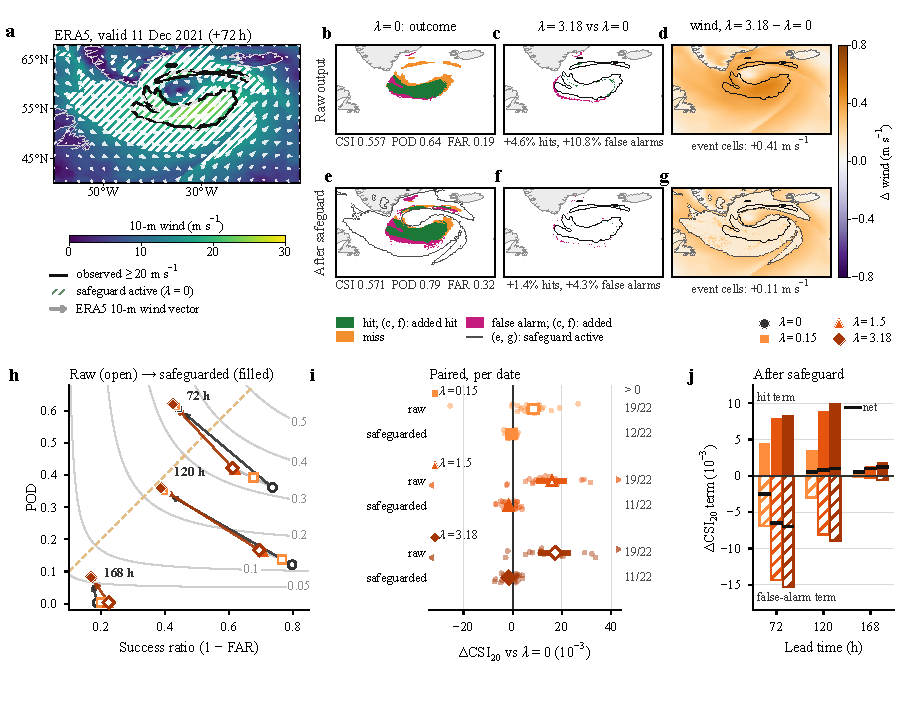
\includegraphics[width=\textwidth]{fig_objective_2021.pdf}
\caption{Event-weighted training and the common safeguard in the objective experiment (2021 cross-year sample, 20 \mps\ wind; colours darken with the event weight $\lambda$). (a--g) ERA5-selected case (largest observed 20 \mps\ area of the 22 dates; 00 UTC 8 December 2021, +72 h): (a) ERA5 wind and vectors, observed events and safeguard-active cells; (b--d) raw output and (e--g) after the safeguard: outcome of $\lambda=0$ (seed 123), cells added by $\lambda=3.18$, and the wind difference $\lambda=3.18$ minus $\lambda=0$ (three-seed mean). (h) Performance diagram of all dates at 72, 120 and 168 h. (i) Paired CSI$_{20}$ differences to $\lambda=0$ with 95\% intervals from date resampling (thick) and 7- and 14-day blocks (thinner); dots are single dates, numbers count positive dates. (j) Hit and false-alarm terms of the safeguarded difference.}
\label{fig:objective}
\end{figure}

\subsection{Limits at 25 \mps\ and computational cost}
\label{sec:limits}

The safeguard can only restore what a member forecasts. Table~S6 decomposes the observed area at or above 25 \mps\ in 2022: at 168 h, 90\% of that area has no member reaching 25 \mps, the two-member consensus fails on 66\%, and the gate is active on only 34\% of the observed event area (95\% at 72 h). The three-seed mean shortfall of the fused forecast on missed cells grows from 4.84 \mps\ at 72 h to 13.43 \mps\ at 168 h, and the share of misses that are near misses in the 20--25 \mps\ band falls from 76\% to 16\%. The 25 \mps\ CSI of PS-PaE-Fuse therefore stays below Pangu-Weather; this is a property of the inputs and of the fixed rule, not a statement about predictability. On the cost side, one global inference of the two experts and the frozen selector for four members, six variables and one lead time takes 0.72 $\pm$ 0.03 s (five timed runs) with 0.86 GiB peak memory on a single NVIDIA RTX 4090, for 558\,239 deployable parameters, excluding disk input and the upstream member forecasts; the safeguard and the linear stacking are negligible in comparison.

\section{Discussion}
\label{sec:discussion}

\subsection{Roles of the learned experts and the safeguard}
\label{sec:roles}

The ablations assign distinct roles to the components of PS-PaE-Fuse. The safeguard sets the operating point for extreme wind: it doubles the alert area to the observed event rate, raises POD and FAR by about 0.2 each and improves the neighbourhood FSS in every season and stratum. This pays for users whose protection cost is below roughly a third to a half of the avoided loss. The frequency-matched control is the most informative comparison, because it separates more alerts from better-placed alerts; the safeguard wins only the second part, by a small and not significant margin in CSI.

The learned experts supply the continuous and probabilistic fields: their U10 RMSE is 16--17\% below Pangu-Weather before the safeguard (14--15\% after it) and comparable to the member mean, and their U10 CRPS and Brier score are lower than those of EMOS. They add no measurable detection once the safeguard is applied, consistent with evidence that data-driven models underestimate extremes and benefit from dedicated post-processing (Trotta et al., 2025; Yuan et al., 2026) and with the forecaster's dilemma (Lerch et al., 2017): a fusion trained on error and probabilistic scores is rewarded for hedging, and reweighting members cannot restore intensity removed by the mean without restoring member placement errors. The phase-aware routing is active in training and changes the network output, but its independent contribution to skill is not established on the present samples.

\subsection{Why event-weighted training and the safeguard do not add up}
\label{sec:interaction}

Both mechanisms act on the same cells. The joint objective raises the fused wind where members agree on strong wind, because an additional 20 \mps\ hit is cheapest there in mean-square error, and the consensus safeguard replaces the fused vector in exactly those cells. Once the rule fires the amplitude increase is redundant, and where it fires on a false alarm the joint model has already moved the wind in the wrong direction, so the false-alarm term of the 72 h decomposition exceeds the hit term. Objectives designed for raw output must therefore be evaluated at the deployed operating point; the soft-CSI loss itself is a standard multi-objective loss. For PS-PaE-Fuse this supports keeping detection in a separate forecast-time module whose operating point can be set and costed explicitly.

\subsection{Limitations}
\label{sec:limitations}

The samples are small and were not untouched: the 2021 sample covers 22 dates of one autumn and the 2022 sample 32 dates spread over one year, both inspected during development of the neural system, so the intervals are pointwise sensitivity intervals of a sparse reused sample, uncorrected for multiple comparisons, rather than confirmatory tests. The routing-feature ablation was run after the 2022 results were known and is exploratory, and the linear objective experiment was run on the 2021 sample only. ERA5 is the verification reference for all systems; it underestimates the most intense winds and is itself a model product, so absolute CSI values at 25 \mps\ are not comparable with station-based scores. Event thresholds, the safeguard trigger and the shared scale were fixed on 2020, and the objective experiment and PS-PaE-Fuse use different safeguard configurations, so the paper does not present one continuous ablation. Detection is assessed for surface wind only, and the six-variable results show mixed changes relative to the simple mean. The upper-air scores of an earlier version of the 2021 evaluation were affected by a valid-time indexing error in the Z500 and T850 reference fields; the objective experiment and Table~S2 use the corrected reference, while the development-only calibration diagnostics in Table~S9 retain the original cached reference; the surface fields were unaffected.

\section{Conclusions}
\label{sec:conclusions}

We introduced PS-PaE-Fuse, an extreme-aware fusion system that turns Pangu-Weather, GraphCast, FuXi and ECMWF HRES into deterministic, probabilistic and event outputs for six variables, and verified it under a protocol frozen on 2020 on 22 dates of 2021 and 32 sealed dates of 2022. Three conclusions follow. First, the complete system improves the detection of local extreme surface wind relative to the best member: on the sealed sample the q97.5 wind CSI rises from 0.286 for Pangu-Weather to 0.344 and the FSS$_{9}$ from 0.603 to 0.678, in every season and in tropical-cyclone, cold-surge and non-tropical high-wind conditions, with 14\% lower U10 RMSE. Second, the ablations identify the roles of the components: the consensus safeguard carries the detection gain, which a member mean with the same rule reproduces and a frequency-matched threshold largely reproduces with more false alarms, whereas the learned experts supply the continuous fields and probabilistic outputs, whose U10 CRPS and Brier score are lower than those of EMOS before the safeguard; the gain doubles the alert area to the observed event rate and degrades the Brier score, of which a shared-scale calibration recovers about one third. Third, event weighting in the loss of a linear stacking raises the raw 20 \mps\ CSI by 0.008--0.017 at an error cost below 0.04\% but is absorbed by the safeguard, so detection-oriented components must be evaluated at the deployed operating point. PS-PaE-Fuse thus gives AI multi-model forecasts an explicit, costed operating point for extreme-wind warnings at sub-second post-processing cost; conditional calibration and members that reach higher wind speeds are the next steps.

\acknowledgmentsname{\todo{Funding, computing resources and individual assistance must be supplied by the authors.} ERA5 is provided by the Copernicus Climate Change Service; IBTrACS by NOAA/NCEI; the Pangu-Weather, GraphCast and FuXi models by their developers.}

\vspace*{3mm}
\noindent{\it Data availability}. Pangu-Weather, HRES and ERA5 were read from the public WeatherBench~2 archive (Rasp et al., 2024), stores \path{pangu/2018-2022_0012_0p25.zarr}, \path{hres/2016-2022-12h-6h-0p25deg-chunk-1.zarr} and \path{era5/1959-2023_01_10-wb13-6h-1440x721_with_derived_variables.zarr} under \path{gs://weatherbench2/datasets/}; IBTrACS v04r01 is available from NOAA/NCEI (Knapp et al., 2010). \todo{Authors must provide the public repository/DOI, access conditions and redistribution permissions for the PS-PaE-Fuse code, frozen checkpoints, thresholds, evaluation records and analysis code. No public deposition has been verified.}

\vspace*{3mm}
\noindent{\it Authors' contributions}. \colorbox{yellow}{To be completed.}

\vspace*{3mm}
\noindent{\it Competing interests}. \todo{Authors must confirm the original declaration: no competing interests.}

\vspace*{3mm}
\noindent{\it Electronic supplementary material}. Supplementary Tables S1--S11 and Fig.~S1 are provided in a separate file.

\begin{Exercises}
\item\hspace*{-6mm}
Allen, S., D. Ginsbourger, and J. Ziegel, 2023: Evaluating forecasts for high-impact events using transformed kernel scores. \textit{SIAM/ASA J. Uncertainty Quantification}, \textbf{11}(3), 906--940, \url{https://doi.org/10.1137/22M1532184}.

\item\hspace*{-6mm}
Ben Bouall\`egue, Z., and Coauthors, 2024: The rise of data-driven weather forecasting: A first statistical assessment of machine learning--based weather forecasts in an operational-like context. \textit{Bull. Amer. Meteor. Soc.}, \textbf{105}(6), E864--E883, \url{https://doi.org/10.1175/BAMS-D-23-0162.1}.

\item\hspace*{-6mm}
Bi, K. F., L. X. Xie, H. H. Zhang, X. Chen, X. T. Gu, and Q. Tian, 2023: Accurate medium-range global weather forecasting with 3D neural networks. \textit{Nature}, \textbf{619}(7970), 533--538, \url{https://doi.org/10.1038/s41586-023-06185-3}.

\item\hspace*{-6mm}
Biegert, T., S. Allen, A. Alber, and S. Lerch, 2026: Towards fair comparisons of AI- and physics-based weather models for extreme events via the weighted potential CRPS. arXiv:2606.21170, \url{https://doi.org/10.48550/arXiv.2606.21170}.

\item\hspace*{-6mm}
Brier, G. W., 1950: Verification of forecasts expressed in terms of probability. \textit{Mon. Wea. Rev.}, \textbf{78}(1), 1--3, \url{https://doi.org/10.1175/1520-0493(1950)078<0001:VOFEIT>2.0.CO;2}.

\item\hspace*{-6mm}
Charlton-Perez, A. J., and Coauthors, 2024: Do AI models produce better weather forecasts than physics-based models? A quantitative evaluation case study of Storm Ciar\'an. \textit{npj Clim. Atmos. Sci.}, \textbf{7}, 93, \url{https://doi.org/10.1038/s41612-024-00638-w}.

\item\hspace*{-6mm}
Chen, K., and Coauthors, 2023b: FengWu: Pushing the skillful global medium-range weather forecast beyond 10 days lead. arXiv:2304.02948, \url{https://doi.org/10.48550/arXiv.2304.02948}.

\item\hspace*{-6mm}
Chen, L., X. H. Zhong, F. Zhang, Y. Cheng, Y. H. Xu, Y. Qi, and H. Li, 2023a: FuXi: A cascade machine learning forecasting system for 15-day global weather forecast. \textit{npj Clim. Atmos. Sci.}, \textbf{6}, 190, \url{https://doi.org/10.1038/s41612-023-00512-1}.

\item\hspace*{-6mm}
Dai, G. K., H. Li, M. Mu, G. H. Wang, B. Qin, X. H. Zhong, F. Zhang, and X. S. Liang, 2026: Artificial intelligence for atmospheric and oceanic forecasting and research: A Fudan University perspective. \textit{Adv. Atmos. Sci.}, in press, \url{https://doi.org/10.1007/s00376-026-6149-7}.

\item\hspace*{-6mm}
Gneiting, T., and A. E. Raftery, 2007: Strictly proper scoring rules, prediction, and estimation. \textit{J. Amer. Stat. Assoc.}, \textbf{102}(477), 359--378, \url{https://doi.org/10.1198/016214506000001437}.

\item\hspace*{-6mm}
Gneiting, T., A. E. Raftery, A. H. Westveld, and T. Goldman, 2005: Calibrated probabilistic forecasting using ensemble model output statistics and minimum CRPS estimation. \textit{Mon. Wea. Rev.}, \textbf{133}(5), 1098--1118, \url{https://doi.org/10.1175/MWR2904.1}.

\item\hspace*{-6mm}
Hagedorn, R., F. J. Doblas-Reyes, and T. N. Palmer, 2005: The rationale behind the success of multi-model ensembles in seasonal forecasting---I. Basic concept. \textit{Tellus A}, \textbf{57}(3), 219--233, \url{https://doi.org/10.1111/j.1600-0870.2005.00103.x}.

\item\hspace*{-6mm}
Hersbach, H., and Coauthors, 2020: The ERA5 global reanalysis. \textit{Quart. J. Roy. Meteor. Soc.}, \textbf{146}(730), 1999--2049, \url{https://doi.org/10.1002/qj.3803}.

\item\hspace*{-6mm}
Jacobs, R. A., M. I. Jordan, S. J. Nowlan, and G. E. Hinton, 1991: Adaptive mixtures of local experts. \textit{Neural Comput.}, \textbf{3}(1), 79--87, \url{https://doi.org/10.1162/neco.1991.3.1.79}.

\item\hspace*{-6mm}
Knapp, K. R., M. C. Kruk, D. H. Levinson, H. J. Diamond, and C. J. Neumann, 2010: The International Best Track Archive for Climate Stewardship (IBTrACS): Unifying tropical cyclone data. \textit{Bull. Amer. Meteor. Soc.}, \textbf{91}(3), 363--376, \url{https://doi.org/10.1175/2009BAMS2755.1}.

\item\hspace*{-6mm}
Krishnamurti, T. N., C. M. Kishtawal, T. E. LaRow, D. R. Bachiochi, Z. Zhang, C. E. Williford, S. Gadgil, and S. Surendran, 1999: Improved weather and seasonal climate forecasts from multimodel superensemble. \textit{Science}, \textbf{285}(5433), 1548--1550, \url{https://doi.org/10.1126/science.285.5433.1548}.

\item\hspace*{-6mm}
Lagerquist, R., and I. Ebert-Uphoff, 2022: Can we integrate spatial verification methods into neural network loss functions for atmospheric science? \textit{Artif. Intell. Earth Syst.}, \textbf{1}(4), e220021, \url{https://doi.org/10.1175/AIES-D-22-0021.1}.

\item\hspace*{-6mm}
Lam, R., and Coauthors, 2023: Learning skillful medium-range global weather forecasting. \textit{Science}, \textbf{382}(6677), 1416--1421, \url{https://doi.org/10.1126/science.adi2336}.

\item\hspace*{-6mm}
Lang, S., and Coauthors, 2024: AIFS -- ECMWF's data-driven forecasting system. arXiv:2406.01465, \url{https://doi.org/10.48550/arXiv.2406.01465}.

\item\hspace*{-6mm}
Lerch, S., T. L. Thorarinsdottir, F. Ravazzolo, and T. Gneiting, 2017: Forecaster's dilemma: Extreme events and forecast evaluation. \textit{Stat. Sci.}, \textbf{32}(1), 106--127, \url{https://doi.org/10.1214/16-STS588}.

\item\hspace*{-6mm}
Li, Y. H., W. S. Duan, H. Li, W. Han, H. Zhang, and Y. N. Li, 2026: A synergistic approach: Dynamics--AI ensemble in tropical cyclone forecasting. \textit{Adv. Atmos. Sci.}, \textbf{43}(9), 1763--1774, \url{https://doi.org/10.1007/s00376-026-5784-3}.

\item\hspace*{-6mm}
Lin, T.-Y., P. Goyal, R. Girshick, K. M. He, and P. Doll\'ar, 2020: Focal loss for dense object detection. \textit{IEEE Trans. Pattern Anal. Mach. Intell.}, \textbf{42}(2), 318--327, \url{https://doi.org/10.1109/TPAMI.2018.2858826}.

\item\hspace*{-6mm}
Liu, C.-C., and Coauthors, 2024: Evaluation of five global AI models for predicting weather in Eastern Asia and Western Pacific. \textit{npj Clim. Atmos. Sci.}, \textbf{7}, 221, \url{https://doi.org/10.1038/s41612-024-00769-0}.

\item\hspace*{-6mm}
Liu, X., and Coauthors, 2025: Global ensemble weather prediction from a deep learning--based model (Pangu-Weather) with the initial condition perturbations of CMA-GEPS. \textit{Adv. Atmos. Sci.}, \textbf{42}(8), 1636--1660, \url{https://doi.org/10.1007/s00376-024-4173-z}.

\item\hspace*{-6mm}
Loshchilov, I., and F. Hutter, 2019: Decoupled weight decay regularization. \textit{Seventh Int. Conf. on Learning Representations (ICLR 2019)}, New Orleans, LA, arXiv:1711.05101, \url{https://doi.org/10.48550/arXiv.1711.05101}.

\item\hspace*{-6mm}
Mass, C. F., D. Ovens, K. Westrick, and B. A. Colle, 2002: Does increasing horizontal resolution produce more skillful forecasts? \textit{Bull. Amer. Meteor. Soc.}, \textbf{83}(3), 407--430, \url{https://doi.org/10.1175/1520-0477(2002)083<0407:DIHRPM>2.3.CO;2}.

\item\hspace*{-6mm}
Mu, M., B. Qin, and G. K. Dai, 2025: Predictability study of weather and climate events related to artificial intelligence models. \textit{Adv. Atmos. Sci.}, \textbf{42}(1), 1--8, \url{https://doi.org/10.1007/s00376-024-4372-7}.

\item\hspace*{-6mm}
Murphy, A. H., 1977: The value of climatological, categorical and probabilistic forecasts in the cost-loss ratio situation. \textit{Mon. Wea. Rev.}, \textbf{105}(7), 803--816, \url{https://doi.org/10.1175/1520-0493(1977)105<0803:TVOCCA>2.0.CO;2}.

\item\hspace*{-6mm}
Nai, C. Y., X. Chen, S. S. Yang, Z. N. Xiao, and B. X. Pan, 2025: Boosting weather forecast via generative superensemble. \textit{npj Clim. Atmos. Sci.}, \textbf{8}, 377, \url{https://doi.org/10.1038/s41612-025-01255-x}.

\item\hspace*{-6mm}
Niu, Z. Y., W. Huang, Y. H. Yang, M. Q. Yang, L. Deng, H. B. Wang, H. Li, and X. Zhang, 2026: Evaluating the Shanghai Typhoon Model against state-of-the-art machine-learning weather prediction models: A case study for Typhoon Danas (2025). \textit{Adv. Atmos. Sci.}, \textbf{43}(4), 744--750, \url{https://doi.org/10.1007/s00376-025-5464-8}.

\item\hspace*{-6mm}
Olivetti, L., and G. Messori, 2024: Do data-driven models beat numerical models in forecasting weather extremes? A comparison of IFS HRES, Pangu-Weather, and GraphCast. \textit{Geosci. Model Dev.}, \textbf{17}(21), 7915--7962, \url{https://doi.org/10.5194/gmd-17-7915-2024}.

\item\hspace*{-6mm}
Pasche, O. C., J. Wider, Z. W. Zhang, J. Zscheischler, and S. Engelke, 2025: Validating deep learning weather forecast models on recent high-impact extreme events. \textit{Artif. Intell. Earth Syst.}, \textbf{4}(1), e240033, \url{https://doi.org/10.1175/AIES-D-24-0033.1}.

\item\hspace*{-6mm}
Pathak, J., and Coauthors, 2022: FourCastNet: A global data-driven high-resolution weather model using adaptive Fourier neural operators. arXiv:2202.11214, \url{https://doi.org/10.48550/arXiv.2202.11214}.

\item\hspace*{-6mm}
Price, I., and Coauthors, 2025: Probabilistic weather forecasting with machine learning. \textit{Nature}, \textbf{637}(8044), 84--90, \url{https://doi.org/10.1038/s41586-024-08252-9}.

\item\hspace*{-6mm}
Rasp, S., and S. Lerch, 2018: Neural networks for postprocessing ensemble weather forecasts. \textit{Mon. Wea. Rev.}, \textbf{146}(11), 3885--3900, \url{https://doi.org/10.1175/MWR-D-18-0187.1}.

\item\hspace*{-6mm}
Rasp, S., and Coauthors, 2024: WeatherBench 2: A benchmark for the next generation of data-driven global weather models. \textit{J. Adv. Model. Earth Syst.}, \textbf{16}(6), e2023MS004019, \url{https://doi.org/10.1029/2023MS004019}.

\item\hspace*{-6mm}
Richardson, D. S., 2000: Skill and relative economic value of the ECMWF ensemble prediction system. \textit{Quart. J. Roy. Meteor. Soc.}, \textbf{126}(563), 649--667, \url{https://doi.org/10.1002/qj.49712656313}.

\item\hspace*{-6mm}
Roberts, N. M., and H. W. Lean, 2008: Scale-selective verification of rainfall accumulations from high-resolution forecasts of convective events. \textit{Mon. Wea. Rev.}, \textbf{136}(1), 78--97, \url{https://doi.org/10.1175/2007MWR2123.1}.

\item\hspace*{-6mm}
Roebber, P. J., 2009: Visualizing multiple measures of forecast quality. \textit{Wea. Forecasting}, \textbf{24}(2), 601--608, \url{https://doi.org/10.1175/2008WAF2222159.1}.

\item\hspace*{-6mm}
Salehi, S. S. M., D. Erdogmus, and A. Gholipour, 2017: Tversky loss function for image segmentation using 3D fully convolutional deep networks. \textit{Machine Learning in Medical Imaging}, Lecture Notes in Computer Science, Springer, 379--387, \url{https://doi.org/10.1007/978-3-319-67389-9_44}.

\item\hspace*{-6mm}
Schaefer, J. T., 1990: The critical success index as an indicator of warning skill. \textit{Wea. Forecasting}, \textbf{5}(4), 570--575, \url{https://doi.org/10.1175/1520-0434(1990)005<0570:TCSIAA>2.0.CO;2}.

\item\hspace*{-6mm}
Schulz, B., and S. Lerch, 2022: Machine learning methods for postprocessing ensemble forecasts of wind gusts: A systematic comparison. \textit{Mon. Wea. Rev.}, \textbf{150}(1), 235--257, \url{https://doi.org/10.1175/MWR-D-21-0150.1}.

\item\hspace*{-6mm}
Trotta, B., and Coauthors, 2025: Statistical postprocessing yields accurate probabilistic forecasts from artificial intelligence weather models. \textit{Artif. Intell. Earth Syst.}, \textbf{4}(4), e250037, \url{https://doi.org/10.1175/AIES-D-25-0037.1}.

\item\hspace*{-6mm}
Vannitsem, S., and Coauthors, 2021: Statistical postprocessing for weather forecasts: Review, challenges, and avenues in a big data world. \textit{Bull. Amer. Meteor. Soc.}, \textbf{102}(3), E681--E699, \url{https://doi.org/10.1175/BAMS-D-19-0308.1}.

\item\hspace*{-6mm}
Wessel, J. B., C. A. T. Ferro, G. R. Evans, and F. Kwasniok, 2025: Improving probabilistic forecasts of extreme wind speeds by training statistical post-processing models with weighted scoring rules. \textit{Mon. Wea. Rev.}, \textbf{153}(8), 1489--1511, \url{https://doi.org/10.1175/MWR-D-24-0151.1}.

\item\hspace*{-6mm}
Wilks, D. S., 1997: Resampling hypothesis tests for autocorrelated fields. \textit{J. Climate}, \textbf{10}(1), 65--82, \url{https://doi.org/10.1175/1520-0442(1997)010<0065:RHTFAF>2.0.CO;2}.

\item\hspace*{-6mm}
Wilks, D. S., 2011: \textit{Statistical Methods in the Atmospheric Sciences}. 3rd ed., Academic Press, 676 pp.

\item\hspace*{-6mm}
Yuan, S. J., G. S. Wang, B. Mu, and F. F. Zhou, 2025: TianXing: A linear complexity transformer model with explicit attention decay for global weather forecasting. \textit{Adv. Atmos. Sci.}, \textbf{42}(1), 9--25, \url{https://doi.org/10.1007/s00376-024-3313-9}.

\item\hspace*{-6mm}
Yuan, S. J., X. Z. Wang, B. Mu, G. S. Wang, Z. Y. Niu, and H. Li, 2026: A deep learning--based bias correction model for tropical cyclone track and intensity towards forecasting of the TianXing large weather model. \textit{Adv. Atmos. Sci.}, \textbf{43}(3), 612--630, \url{https://doi.org/10.1007/s00376-025-4520-8}.

\item\hspace*{-6mm}
Zheng, Y. G., and Coauthors, 2026: A forecasting paradigm shift: From traditional methods to physics--AI combination in China's national-level severe convective weather operations. \textit{Adv. Atmos. Sci.}, \textbf{43}(10), 2112--2134, \url{https://doi.org/10.1007/s00376-025-5487-1}.

\end{Exercises}

\end{document}
